\documentclass{article}
\usepackage[utf8]{inputenc}
\usepackage{hyperref}
\usepackage{graphicx}
\usepackage{caption} 

\title{CSI5386 : Natural Language Processing \\ Automated Image Captioning Web System}
\author{Lingfeng Zhang 300134245 Ottawa University \and
Yu Sun 8472921 Carleton University}
\date{April 2020}

\begin{document}

\maketitle

GitHub: \href{https://github.com/RichardChangCA/CSI_5386_NLP_Project}{\url{https://github.com/RichardChangCA/CSI_5386_NLP_Project}}

\section{Introduction}
Currently, natural language processing(NLP) and computer vision(CV) are two main branches in artificial intelligence. With the development of deep learning, variants of convolutional neural network(CNN) and recurrent neural network(RNN) are used in these two research fields and are widely used for image classification and object detection in CV, as well as semantic analysis and text generation in NLP. Moreover, combining NLP and CV is a hot research area recently, especially image captioning as well as video storytelling are two related research topics. This work has brought a great challenge to both computer vision and natural language processing communities recently. Like in image captioning, the machine should not only concern about the object in the image, but also the relation between objects, and use human-friendly language to describe the whole image.

In real our life, after posting a picture in social media, we also eager to make some descriptions for it. It costs a lot of time to choose the proper descriptions, so we plan to implement a tool(more specific, a web system) to generate natural language descriptions for visual content like pictures. Besides, many other scenarios can also apply this method like generating real-time command for self-driving cars based on street image and helping search engine process the image information to build the index\cite{goodrum2000image}. To implement these functions, the key feature is related to that how machines understand an image.

Considering previous motivation of image captioning, in the final project, we are going to build a web system that can automatically generate natural language description for the image. In the whole system, the core component is building an image captioning model to process the image and whether the description is suitable or not will affect the system's effectiveness and usability. So, we first do some research about the related works and then design and implement the system. Besides, to prove the efficiency of the model, we also do some experiments and the evaluation by the metrics. Finally, we are going to demonstrate the system for the end-user.

\section{Related Work}
About image captioning, there are three well-studied approaches to automatic image captioning: retrieval based image captioning, template based image captioning, and deep neural network based image captioning\cite{survey2018}. Moreover, each approach can be divided into some subcategories based on the specific method and framework.

In terms of the retrieval based model, Hodosh et al.\cite{hodosh2013framing} establish a framework for sentence-based image description by ranking a given pool of captions. Ordonez et al.\cite{ordonez2011im2text} used 1 Million Captioned Photographs associated with human-generated description to develop an automatic image description method by filtering and retrieving. The advantage of retrieval-based methods is that always return well-formed human-written captions, but in some conditions, these captions may not be able to describe the image properly.

Another method is called the template based model, generating caption through a syntactically and semantically constrained process. Yang et al.\cite{yang2011corpus} first extracted nouns, verbs, scenes, and prepositions from the image then used these to generate the sentence by the statistical language model. Li et al.\cite{li2011composing} used a similar method, the whole process can be divided into two steps, phrase selection and phrase fusion. Compared with the retrieval based model, the caption generated by this approach is more relevant, but the sentence is usually simple and less creative.

Besides, with the development of the neural network, some generation method like seq-2-seq model has been used to solve this problem, motivated by the neural machine translation. Kiros et al. \cite{kiros2014unifying} brought the encoder-decoder framework into
image captioning area by unifying joint image-text embedding
models through multimodal neural language models. Vinyals et al.\cite{vinyals2015show} used to CNN as encoder and LSTM as decoder for image captioning, by the pre-trained image representation and treating the last hidden layer as input to the decoder. Fang et al.\cite{fang2015captions} presents a compositional approach combining visual detectors, language models, and multimodal similarity models for automatically generating image descriptions, learning directly from a dataset of image captions. You et al.\cite{you2016image} proposes a new image captioning approach that combines the top-down and bottom-up approaches through a semantic attention model. 

Since deep learning structure is the black box and we cannot understand and control its processing, Marcella et al.\cite{cornia2019show} proposes a novel image captioning method which can generate diverse descriptions by allowing both grounding and controllability. Moreover, if people want to get a paragraph that contains more than one sentence, the above methods cannot generate diverse sentences, which meaning generating repeated sentences. Hence, Luck et al.\cite{melas2018training} raises a method that can generate sentences with diversity and can combine these sentences into a whole paragraph organically.

Automatic image captioning is a relatively new task, the network with encoder and decoder is widely used in this area, currently. Besides, some improvement tricks like attention mechanisms used in other areas like machine translation can also apply in image captioning.

\section{System Framework}
The whole web system framework is illustrated Figure \ref{fig1} which contains two main components, including UI layer and model layer.

\begin{figure}[h]
\centering
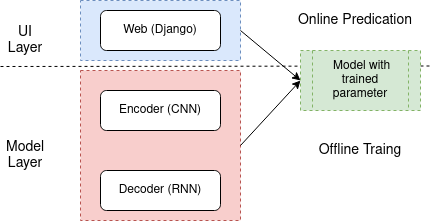
\includegraphics[width=1\textwidth]{framework.png}
\caption{the Framework of Automated Image Captioning Web System}
\label{fig1}
\end{figure}

For the UI layer, we implemented a web system to interact with end-user used Django, and in Model Layer build a generic encoder-decoder model combining some CNN architectures and RNN architectures. Besides, the deep learning model is mainly for offline training and yields a well-train model by serialization, while the UI model loads the model and call the predication method to process user request online. The real application, the model should go through complete training and evaluating offline then can be released online. 

\subsection{UI Layer}
The main function of this component is processing the user's submitted image and displaying a generated description of the image. The layer is relatively lightweight and can be updated iteratively. Besides, the key features of this component are usability and system stability. So, we used Django to develop a web system, which is an open-sourced MVC(Model, View, and Controller) framework for Python. It can make the code more readable as well as decoupled, and can shorten the software development cycle in total, which has been widely used in the industrial area.

\subsection{Model Layer}
In the model layer, it is mainly to build our image captioning neural network model. We used the common sequence-to-sequence with the 4 kinds of CNN architectures as the encoders and the 2 kinds of RNN architectures as the decoders. After comparing their metrics, we finally chose one encoder and one decoder with the best performance as the final prediction model.

\begin{figure}[h]
\centering
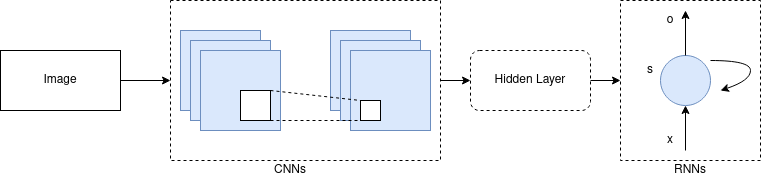
\includegraphics[width=1\textwidth]{model.png}
\caption{The Overview of Model Layer}
\label{fig2}
\end{figure}

For the CNN encoders, we used 4 kinds of pre-trained iamge processing models, including VGG16\cite{simonyan2014very},InceptionV3\cite{szegedy2016rethinking},MobileNet\cite{howard2017mobilenets} and ResNet\cite{he2016deep}, to extract features from images into the hidden layer. For RNN decoders, we tried 2 common used models, including stacked LSTM and GRU with attention mechanism, to generate natural language description of the image from hidden layer. So, we got 8 models in total, which are summarized in the Table \ref{tab1}. Through the whole model, we can get natural language sentences directly from visual data without any other steps.

\begin{table}[htbp]
\centering
\caption{The Summary of All Models}\label{tab1}
\resizebox{\columnwidth}{!}{\begin{tabular}{|l|l|l|l|l|l|l|l|l|l|}
\hline
No. & encoder & decoder \\
\hline
1& InceptionV3 & GRU with Bahdanau Attention\\
2 & MobileNetV2 & GRU with Bahdanau Attention\\
3 & ResNet50 & GRU with Bahdanau Attention\\
4& VGG16 & GRU with Bahdanau Attention\\
5& InceptionV3 & three stacked LSTM\\
6& MobileNetV2 & three stacked LSTM\\
7& ResNet50 & three stacked LSTM\\
8& VGG16 & three stacked LSTM\\
\hline
\end{tabular}}
\end{table}

InceptionV3\cite{szegedy2016rethinking} uses a lot of tricks. Firstly, 1$\times$1 convolution increases the effect of non-linearity and reduces the dimensionality of models to reduce computation. Global average pooling is used in the last layer, instead of fully connected layer to reduce the number of parameters and less prone to overfitting. Intermediate softmax result as auxiliary classifier to minimize weighted loss function, batch normalization and label smoothing can perform as regularization. In addition, factorizing convolution to reduce the number of parameters is another important feature in InceptionV3. Moreover, InceptionV3 also uses grid size reduction to replace max pooling to reserve information of images. MobileNet\cite{howard2017mobilenets} uses depthwise separable convolution to reduce the model size and complexity, which is a light-weight model. However, in most cases, depthwise separable convolution in MobileNet cannot perform better than the standard convolution. ResNet\cite{he2016deep} converges faster and tackles the problem of gradient vanishing and exploding because of its residual connection. This residual architecture ensures the deeper model can outperform shallow models because the function of the residual block is $F(x)=H(x)-x$. If the model reaches the optima, F(x) will be 0, meaning residual architecture can automatically determine the depth of deep learning models. VGGNet\cite{simonyan2014very} uses 3$\times$3 filters and multi-scale training $\&$ testing first, as well as replaces fully-connected layers with convolutional layers to improve the performance.

\begin{figure}[h]
\centering
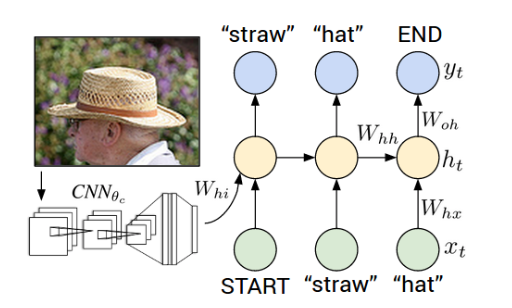
\includegraphics[width=0.7\textwidth]{encoder_decoder.png}
\caption{The intuitive architecture of image captioning encoder-decoder model}
\label{fig_encoder_decoder}
\end{figure}

For encoders, we used pre-trained models with transfer learning and deleted the last fully connected layer as the feature extractor. For decoders, attention mechanism in GRU can predict the next caption word based on the image with certain attention areas and previous caption words context. In addition, stacked LSTM can apply deeper structure to predict captions because the deeper model structure, the better prediction performance in deep learning field in most cases. 

For image captioning task, encoder can extract features from images with the help of convolutional neural network. These features can work as initial hidden state to feed into the RNN decoder. With the start token, the decoder can predict the next caption word one by one until meeting the end token. In training step, after one word is generated, the RNN will move into the next unit and the input of next unit is the original word in previous unit position from the dataset caption which related to this certain image. In predicting step, after one word is generated, the input of next unit is the predicted word in the previous unit. So there is a small difference between training and predicting steps.

\section{Model Evaluation}
Before system is released, we trained the model offline and evaluated it by test data. There are two datasets and three main evaluation metrics, we used for whole evaluation.

\subsection{Dataset}
\begin{enumerate}
\item flickr8k: a small benchmark collection for sentence-based image description, consisting of 8,000 images that are each paired with five different captions. The images were chosen from six different Flickr groups with a variety of scenes and situations.
\item Microsoft COCO: a relatively big benchmark collection for image captioning and related areas, consisting more than 120,000 images and 80 object categories in total. The images are coming from the real life and image backgrounds are more complex.
\end{enumerate}

\subsection{Metric}
For the evaluation, we mainly used three automatic measures, including BLEU, METEOR and CIDEr.
\begin{enumerate}
\item BLEU\cite{papineni2002bleu}: analysing the co-occurrences of n-grams between the candidate and reference sentences, which can be calculated by follow formulas, specially BLEU-1, BLEU-2, BLEU-3 and BLEU-4 are commonly used.
\begin{equation}
C P_{n}(C, S)=\frac{\sum_{i} \sum_{k} \min \left(h_{k}\left(c_{i}\right), \max _{j \in m} h_{k}\left(s_{i j}\right)\right)}{\sum_{i} \sum_{k} h_{k}\left(c_{i}\right)}
\end{equation}
\begin{equation}
b(C, S)=\left\{\begin{array}{ll}
1 & \text { if } l_{C}>l_{S} \\
e^{1-l_{S} / l_{C}} & \text { if } l_{C} \leq l_{S}
\end{array}\right.
\end{equation}
\begin{equation}
BLEU_{N}(C, S)=b(C, S) \exp \left(\sum_{n=1}^{N} w_{n} \log C P_{n}(C, S)\right)   
\end{equation}

\item METEOR\cite{denkowski2014meteor}: calculated by using an alignment between the candidate and reference sentences. The related formulas are listed below:
\begin{equation}
Pen=\gamma\left(\frac{c h}{m}\right)^{\theta} \\
\end{equation}
\begin{equation}
F_{\text {mean}}=\frac{P_{m} R_{m}}{\alpha P_{m}+(1-\alpha) R_{m}} \\
\end{equation}
\begin{equation}
P_{m}=\frac{|m|}{\sum_{k} h_{k}\left(c_{i}\right)} \\
\end{equation}
\begin{equation}
R_{m}=\frac{|m|}{\sum_{k} h_{k}\left(s_{i j}\right)} \\
\end{equation}
\begin{equation}
METEOR=(1-\text {Pen}) F_{\text {mean}} \\
\end{equation}

\item CIDEr\cite{vedantam2015cider}:mainly used in the image captioning, applying the TF-IDF as weight for each n-gram, then calculating the similarity between the candidate and reference sentences by cosine similarity. The related formulas are listed below:
\begin{equation}
\begin{array}{l}
g_{k}\left(s_{i j}\right)= \\
\frac{h_{k}\left(s_{i j}\right)}{\sum_{\omega_{l} \in \Omega} h_{l}\left(s_{i j}\right)} \log \left(\frac{|I|}{\sum_{I_{p} \in I} \min \left(1, \sum_{q} h_{k}\left(s_{p q}\right)\right)}\right)
\end{array}
\end{equation}
\begin{equation}
\operatorname{CIDEr}_{n}\left(c_{i}, S_{i}\right)=\frac{1}{m} \sum_{j} \frac{\boldsymbol{g}^{\boldsymbol{n}}\left(c_{i}\right) \cdot \boldsymbol{g}^{\boldsymbol{n}}\left(s_{i j}\right)}{\left\|\boldsymbol{g}^{\boldsymbol{n}}\left(c_{i}\right)\right\|\left\|\boldsymbol{g}^{\boldsymbol{n}}\left(s_{i j}\right)\right\|} 
\end{equation}
\begin{equation}
\operatorname{CIDEr}\left(c_{i}, S_{i}\right)=\sum_{n=1}^{N} w_{n} \operatorname{CIDEr}_{n}\left(c_{i}, S_{i}\right)
\end{equation}

\end{enumerate}

\subsection{Result Discussion}

Based on previous two datasets, we evaluated each pair of the encoder and the decoder. The whole result and the loss graph are summarised below:

\begin{figure}[h]
\centering
\subfigure{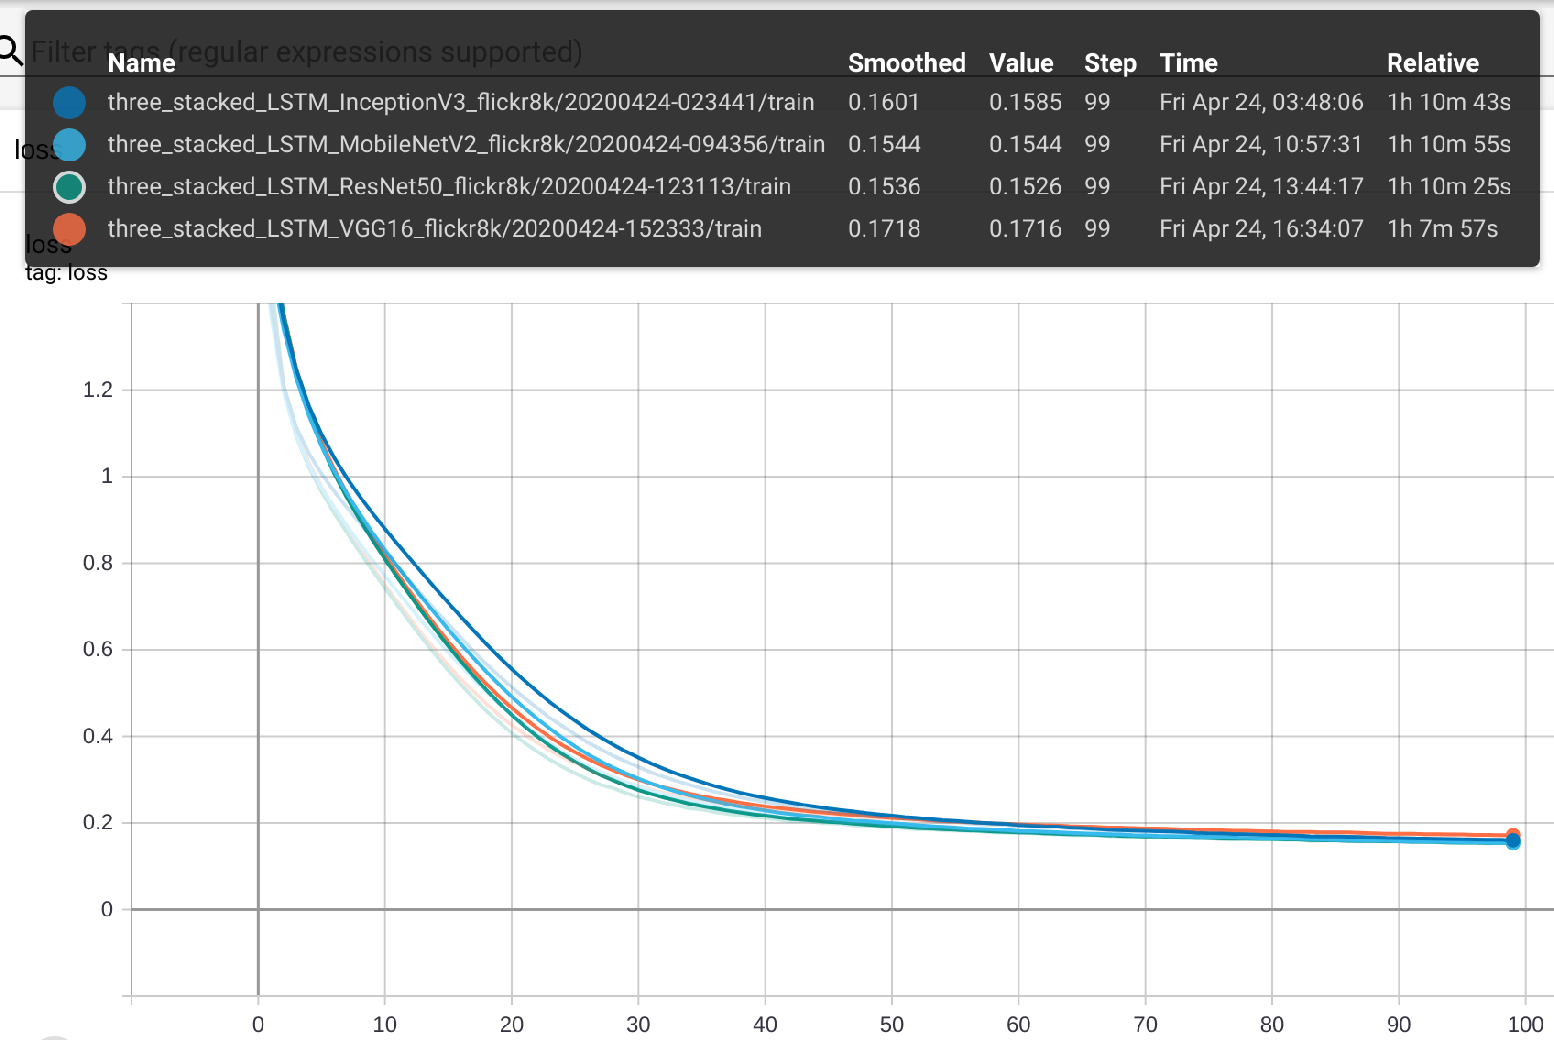
\includegraphics[width=0.415\textwidth]{loss1.png}}
\subfigure{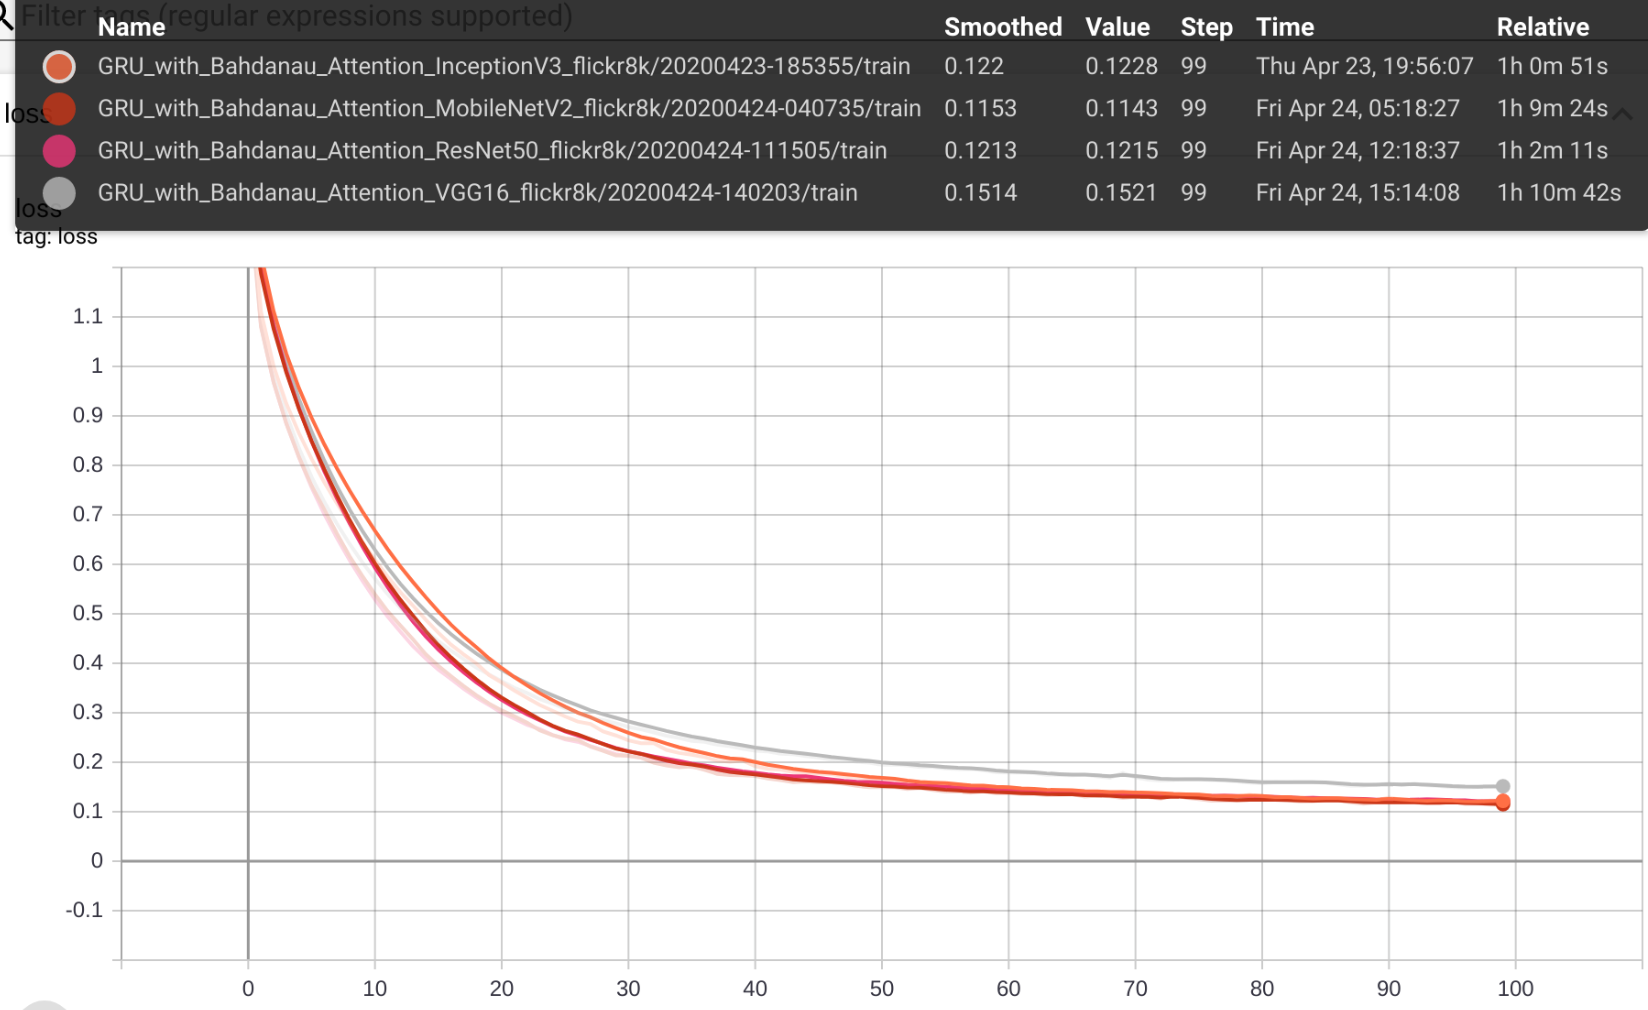
\includegraphics[width=0.45\textwidth]{loss2.png}}
\caption{The Loss Graph for Flickr8k}
\label{fig3}
\end{figure}

\begin{figure}[h]
\centering
\subfigure{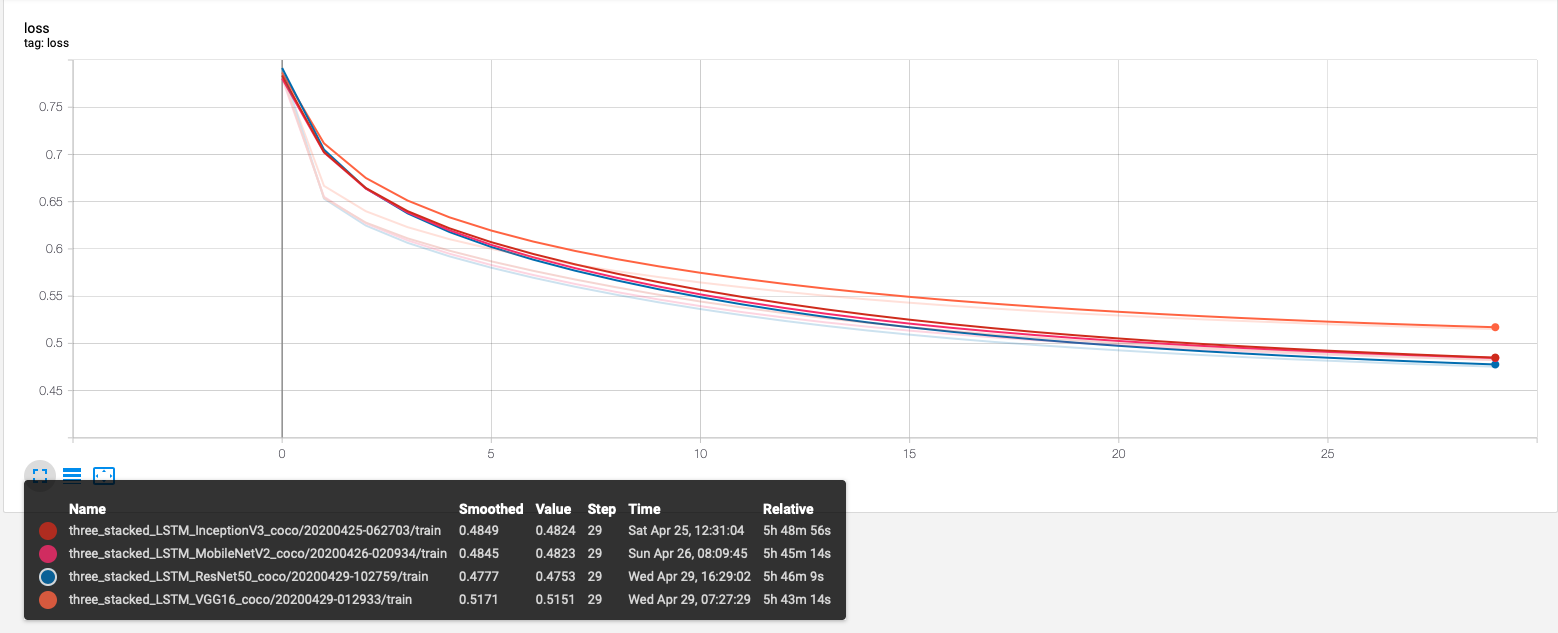
\includegraphics[width=0.43\textwidth]{loss3.png}}
\subfigure{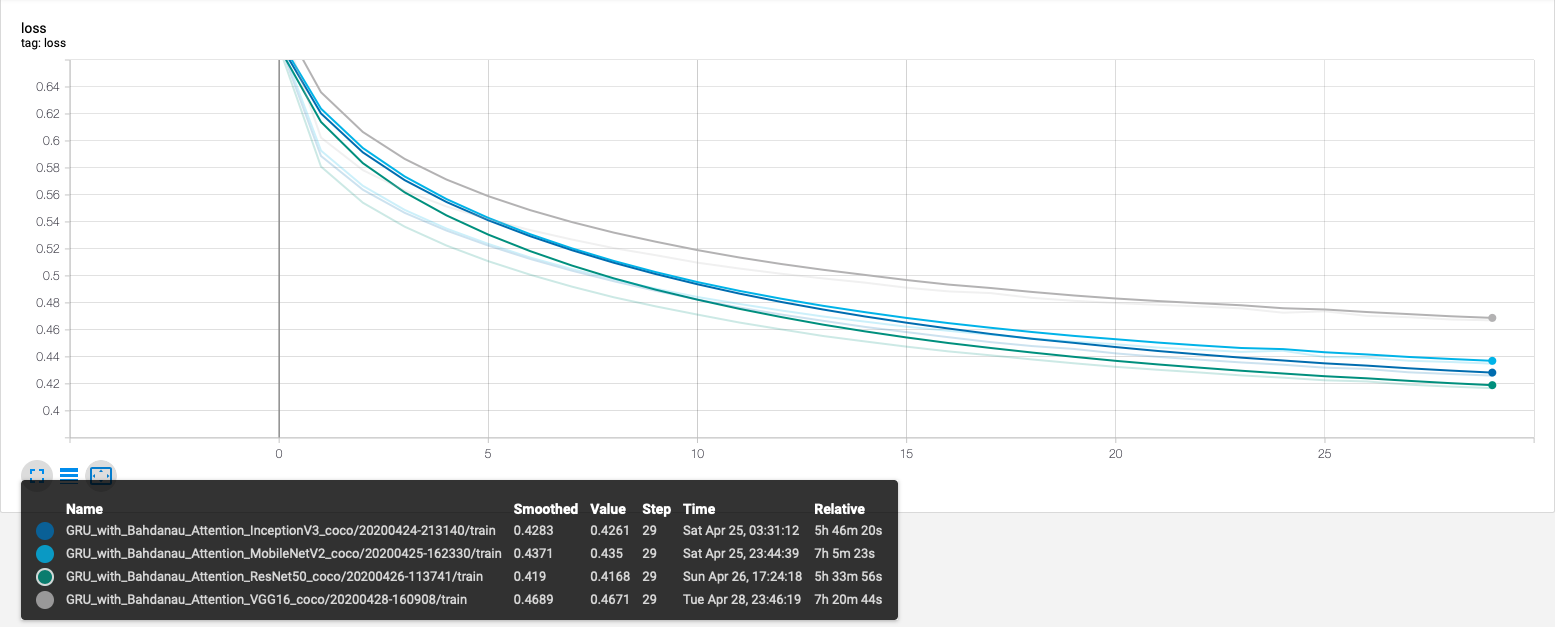
\includegraphics[width=0.43\textwidth]{loss4.png}}
\caption{The Loss Graph for COCO}
\label{fig3_}
\end{figure}

\begin{figure}[h]
\centering
\subfigure{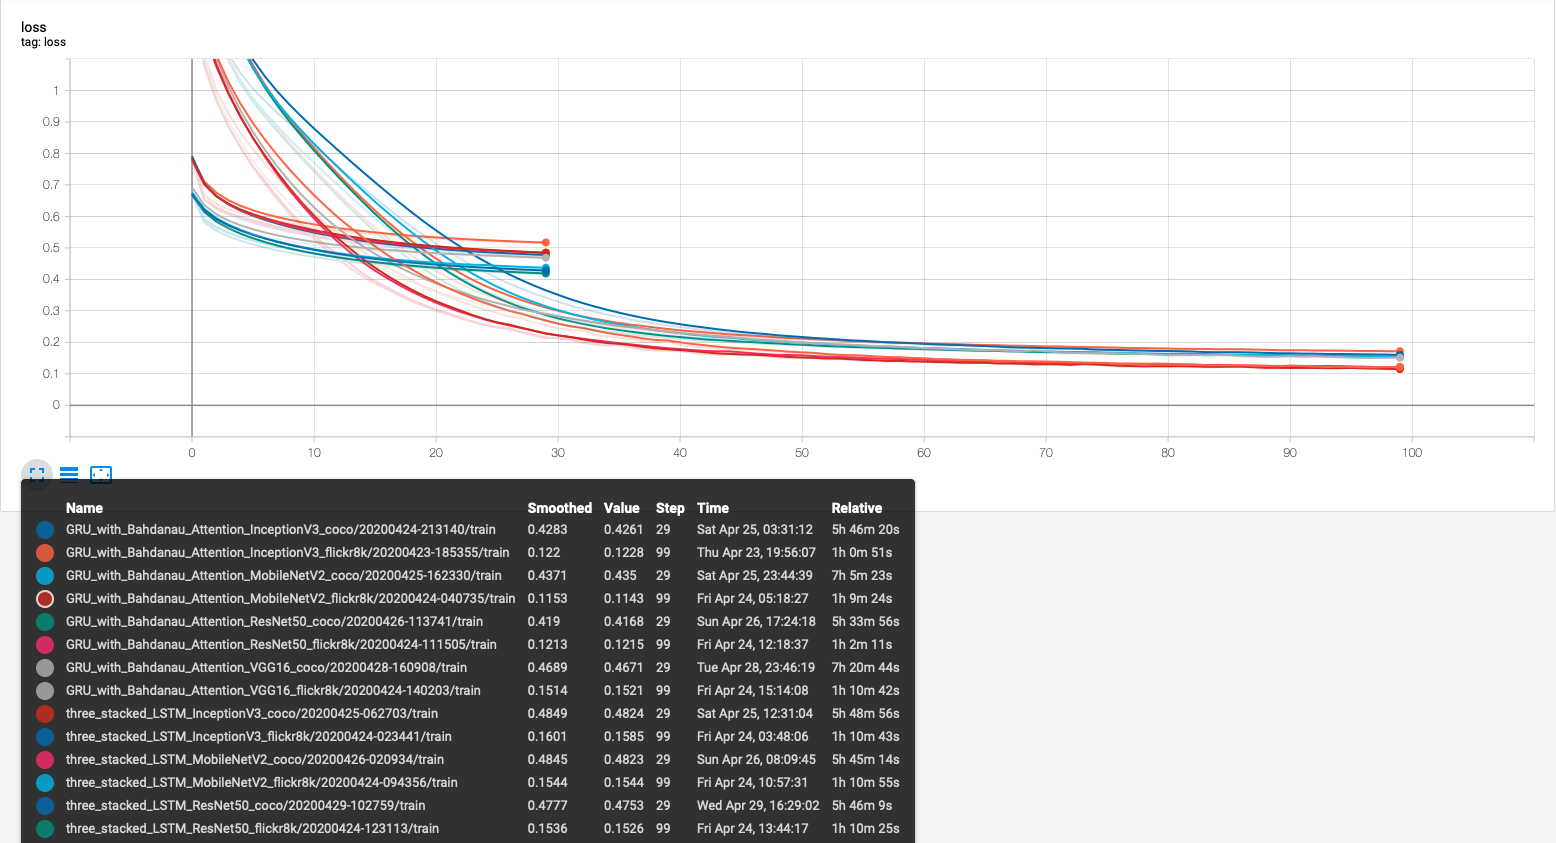
\includegraphics[width=0.7\textwidth]{total_loss.png}}
\caption{The Loss Graph}
\label{_fig3_}
\end{figure}

Overall, we can see loss values in coco dataset are higher than that in flickr8k. Since the size of coco dataset is much larger than that of flickr8k dataset, models trained on coco dataset can converge in small epochs. So we set the epoch to train coco dataset and flickr8k dataset is 30 and 100 respectively.

\begin{table}[htbp]
\centering
\caption{The Evaluation Result}\label{tab2}
\resizebox{\columnwidth}{!}{\begin{tabular}{|l|l|l|l|l|l|l|l|l|l|}
\hline
dataset & encoder & decoder & 1-gram & 2-gram & 3-gram & 4-gram & comulative & CIDEr & METEOR\\
&  &  &blue  & blue &blue & blue  &  blue &  & \\
\hline
flickr8k& InceptionV3 & GRU with Bahdanau Attention & 0.2615 & 0.0754 & 0.0240 & 0.0075 & 0.0784 & 0.5902 & 0.3289\\
flickr8k & MobileNetV2 & GRU with Bahdanau Attention & 0.2599 & 0.0736 & 0.0241 & 0.0077 & 0.0779 & 0.5799 & 0.3232\\
flickr8k & ResNet50 & GRU with Bahdanau Attention & \textbf{0.2646} & \textbf{0.0774} & \textbf{0.0250} & \textbf{0.0084} & \textbf{0.0809} & \textbf{0.6116} & \textbf{0.3295}\\
flickr8k& VGG16 & GRU with Bahdanau Attention & 0.2484 & 0.0688 & 0.0216 & 0.0069 & 0.0725 & 0.5518 & 0.3169\\
flickr8k& InceptionV3 & three stacked LSTM & 0.2309 & 0.0640 & 0.0192 & 0.0057 & 0.0660 & 0.4935 & 0.2994\\
flickr8k& MobileNetV2 & three stacked LSTM & 0.2321 & 0.0651 & 0.0192 & 0.0056 & 0.0664 & 0.4986 & 0.3071\\
flickr8k& ResNet50 & three stacked LSTM & 0.2349 & 0.0662 & 0.0202 & 0.0060 & 0.0683 & 0.4989 & 0.3077\\
flickr8k& VGG16 & three stacked LSTM & 0.2294 & 0.0626 & 0.0181 & 0.0056 & 0.0645 & 0.4882 & 0.3024\\
coco & InceptionV3 & GRU with Bahdanau Attention & 0.1707 & 0.0150 & 0.0017 & 0.0004 & 0.0176 & 0.0482 & 0.1824\\
coco & MobileNetV2 & GRU with Bahdanau Attention & 0.1650 & 0.0140 & 0.0014 & 0.0003 & 0.0159 & 0.0401 & 0.1789\\
coco & ResNet50 & GRU with Bahdanau Attention & 0.1711 & 0.0150 & 0.0016 & 0.0004 & 0.0175 & 0.0452 & 0.1835\\
coco & VGG16 & GRU with Bahdanau Attention & 0.1669 & 0.0145 & 0.0015 & 0.0003 & 0.0166 & 0.0406 & 0.1803\\
coco & InceptionV3 & three stacked LSTM & 0.1526 & 0.0146 & 0.0018 & 0.0003 & 0.0168 & 0.0371 & 0.1691\\
coco & MobileNetV2 & three stacked LSTM & 0.1515 & 0.0141 & 0.0015 & 0.0003 & 0.0159 & 0.0334 & 0.1685\\
coco & ResNet50 & three stacked LSTM & 0.1513 & 0.0128 & 0.0012 & 0.0002 & 0.0140 & 0.0272 & 0.1670\\
coco & VGG16 & three stacked LSTM & 0.1524 & 0.0133 & 0.0012 & 0.0002 & 0.0139 & 0.0278 & 0.1677\\
\hline
\end{tabular}}
\end{table}

According to the evaluation result, the model trained on flickr8k dataset with ResNet50 encoder and Gated Recurrent Unit with Bahdanau Attention mechanism performs the best in this project, with the highest metric scores. So, we decide to apply this well-trained model in the Django automatic image captioning web system.

\subsection{Predication Demo in Web}
The main page of the system allows the user to submit an image, after that, the system will calculate a caption for the image by the trained model.

\begin{figure}[h]
\centering
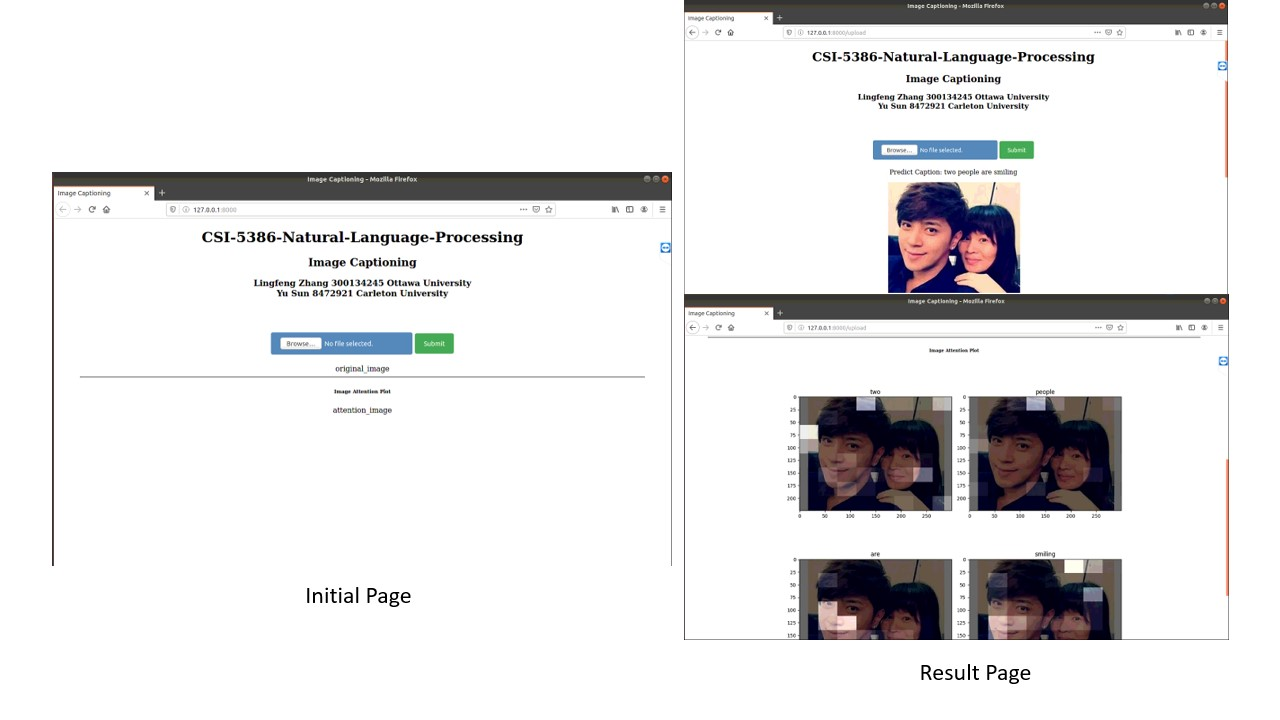
\includegraphics[width=1\textwidth]{system.jpg}
\caption{The System Demo of Predication}
\label{fig4}
\end{figure}

\section{Conclusion}
Motivated by the widely used of image captioning, we build a automated image captioning web system to fulfil the task. Considering the usability, the whole system is divided into two layer, including UI Layer and Model Layer. For the core model, we used 8 kinds of models with different CNN encoders and RNN decoders. 

After the evaluation of these models, we can see the model trained on flickr8k dataset with ResNet50 encoder and GRU with attention mechanism performs the best in this project, probably because of several reasons. The first reason is that ResNet50 convolutional neural network architecture is deep enough to extract features well from images and it can reduce the probability of gradient vanishing problem because of its residual connection. Secondly, attention mechanism can help GRU model to focus on certain areas in images, combined with previous word context, to predict the next word, which is more accurate than models without attention mechanism.

\section{Future Work}

For future work, we plan to fine-tune our model hyper-parameters and structures to find the best result model. In addition, we should increase the number of epoch to train a well-converged model because the training time in this image captioning model is long and we have not sufficient time to train it with very large epoch in this project. Moreover, we also plan to use transformer, bert or other self-attention models to generate more accurate captions. Apart from that, finding a better encoder to extract features better is also important. 

\bibliography{natbib}

\bibliographystyle{ieeetr}

\section{Appendix}

There are two predicted captions for two different images.

\begin{figure}[h]
\centering
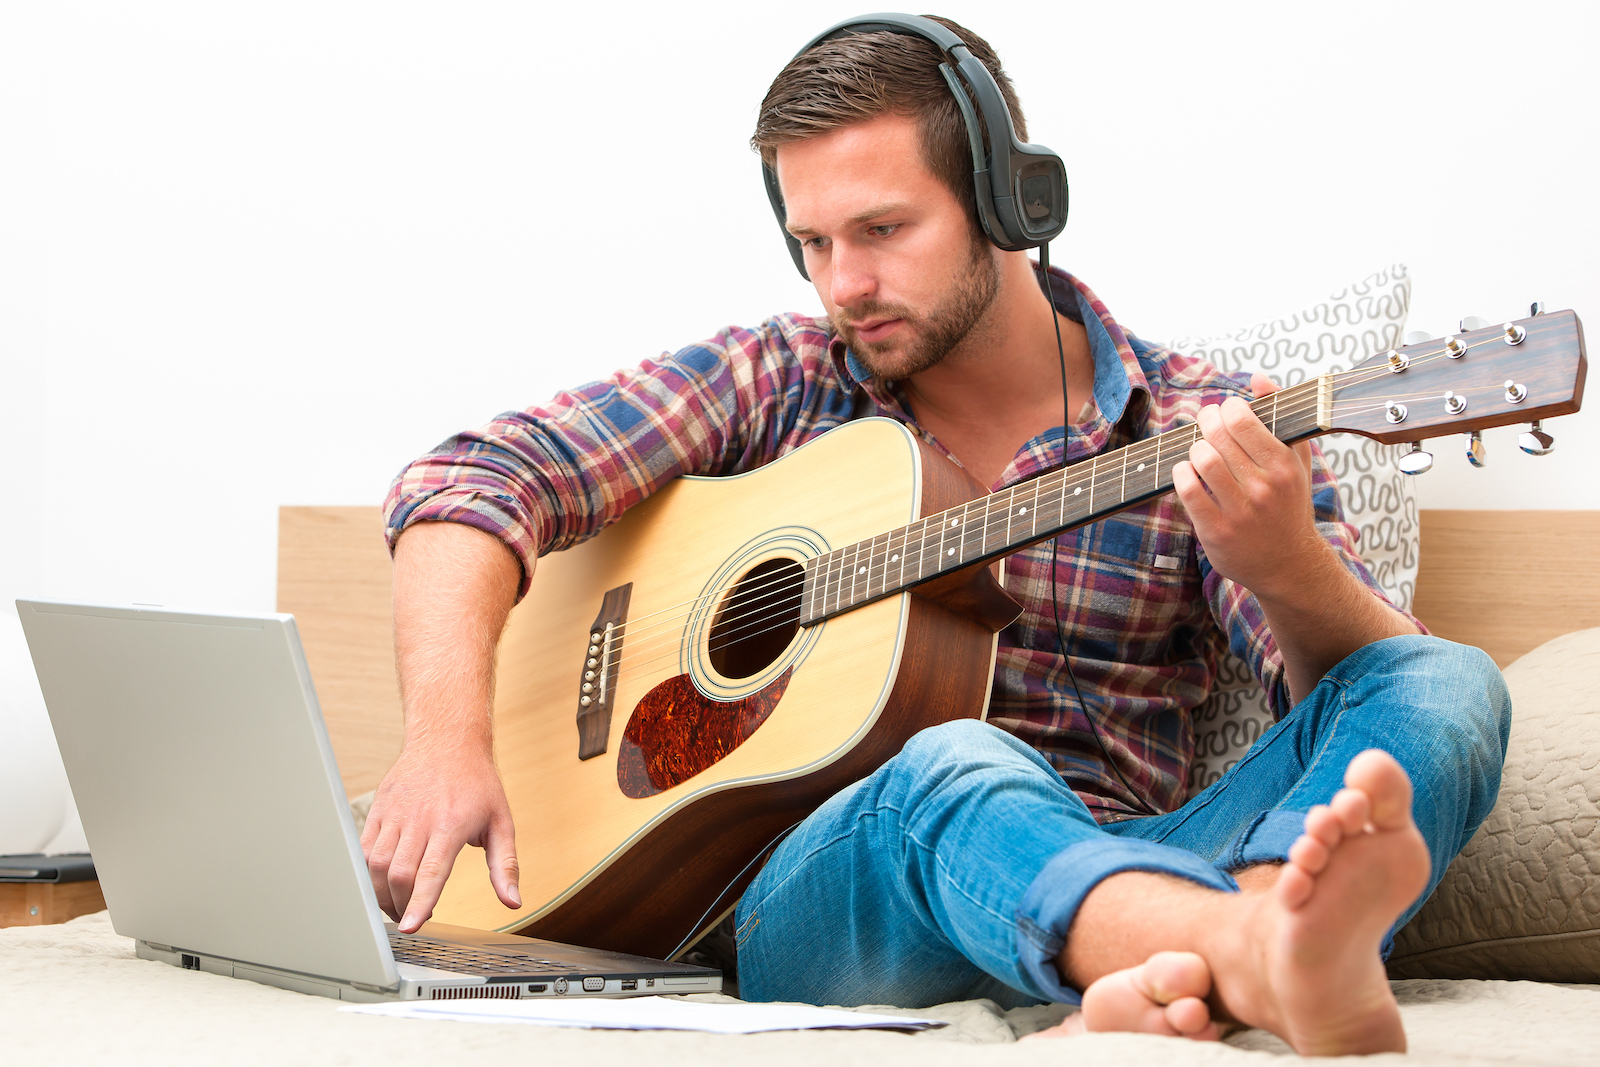
\includegraphics[width=0.5\textwidth]{guitar_man.jpg}
\caption{guitar man}
\label{fig5}
\end{figure}

\begin{figure}[h]
\centering
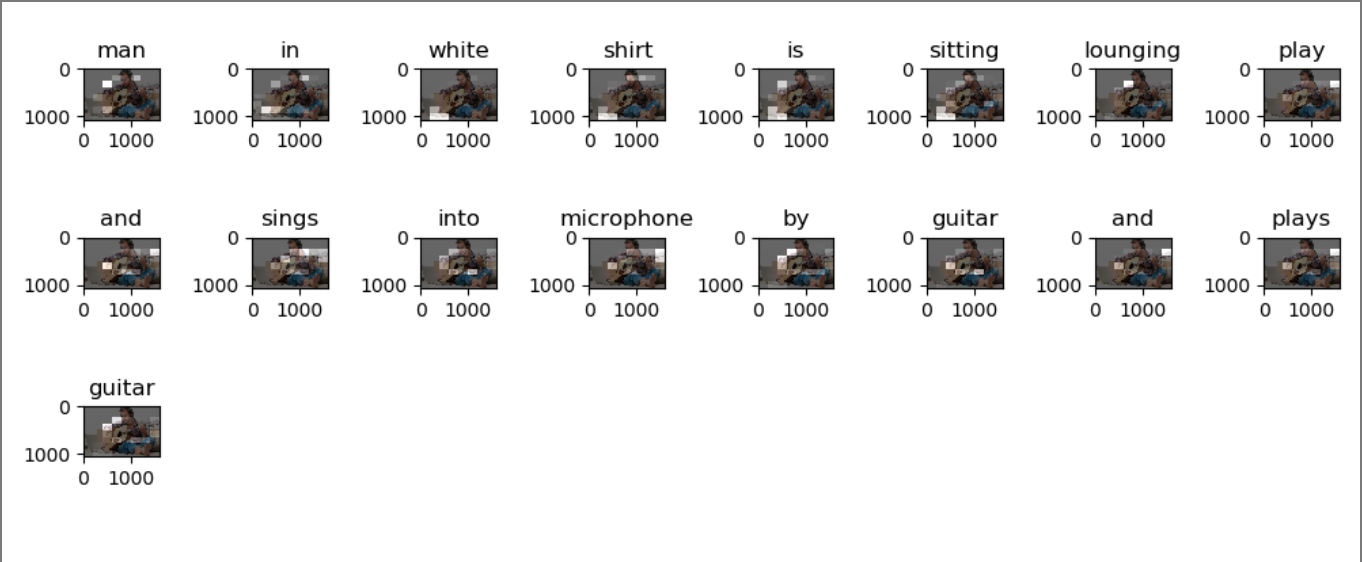
\includegraphics[width=1\textwidth]{attention_plot_guitar_man.png}
\caption{guitar man attention plot}
\label{fig6}
\end{figure}

The predicted caption of the first guitar man image is: man in white shirt is sitting lounging play and sings into microphone by guitar and plays guitar. Each word in this predicted caption focuses on part of images, which means this image captioning model pay more "attention" on part of the image, rather than the whole image for each word one by one during prediction.

The man wears plaid shirt but the shirt color in the predicted caption is white. According to the attention plot, the model focuses on wrong attention area, where the background color is white. Although the man wears earphone with microphone, rather than a single microphone, but this small error does not matter. In addition, this caption has some grammatical error, but you can understand the whole sentence overall.

\begin{figure}[h]
\centering
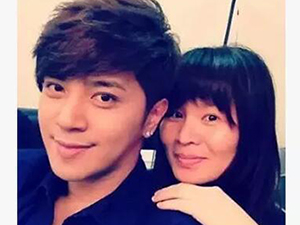
\includegraphics[width=0.5\textwidth]{luozhixiang.jpg}
\caption{two people}
\label{fig7}
\end{figure}

\begin{figure}[h]
\centering
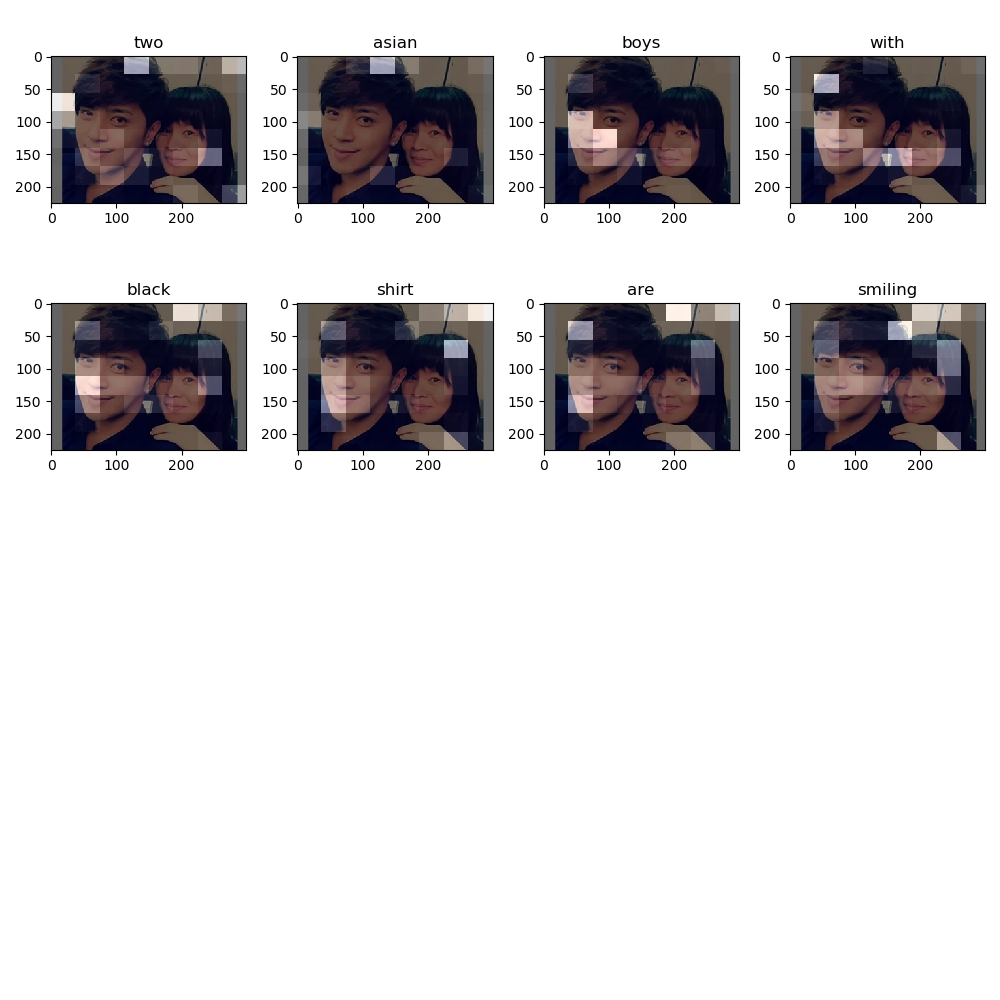
\includegraphics[width=0.5\textwidth]{attention_plot.png}
\caption{two people attention plot}
\label{fig8}
\end{figure}

The predicted caption for the second image is: two Asian boys with black shirt are smiling. Actually one person in the image is man and another person is women, but the model can predict they are Asian. In addition, I guess the word "black" represents their hair color rather than their shirt color although their shirt color is also black.

\end{document}
